Необходимо узнать (проверить) версию системы (Raspbian) с помощью команды (рис.~\ref{driver_1:driver_1}):

\begin{verbatim}
$ uname -a
\end{verbatim} 
 
Далее проверить список доступных USB-устройств (рис.~\ref{driver_1:driver_1}). Запись <<ID 0BDA:8179>> и версия ОС будут определять, какой драйвер необходим. 

\begin{figure}[h!]
\center{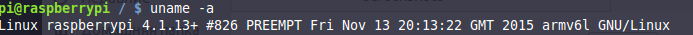
\includegraphics[width=0.8\linewidth]{driver_1}}
\caption{ Текущая версия системы }
\label{driver_1:driver_1}
\end{figure}


\begin{figure}[h!]
\center{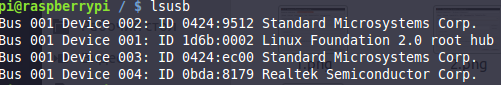
\includegraphics[width=0.5\linewidth]{driver_2}}
\caption{ Список USB-устройств }
\label{driver_2:driver_2}
\end{figure}

Подробную инструкцию можно найти, перейдя по ссылке \cite{rpi-tp}.

Остается загрузить необходимый драйвер (рис.~\ref{driver_3:driver_3}), установить его и перезагрузиться (рис.~\ref{driver_4:driver_4}). В случае успешной установки драйвера, команда ifconfig отобразит наличие беспроводного соединения wlan0 (рис.~\ref{driver_5:driver_5}).

\begin{figure}[h!]
\center{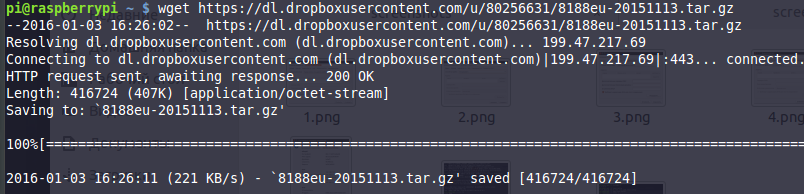
\includegraphics[width=0.8\linewidth]{driver_3}}
\caption{ Загрузка драйвера }
\label{driver_3:driver_3}
\end{figure}

\begin{figure}[h!]
\center{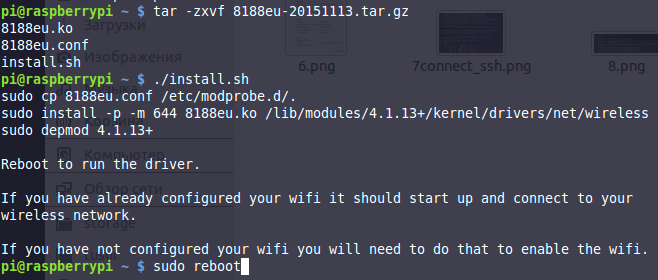
\includegraphics[width=0.6\linewidth]{driver_4}}
\caption{ Установка драйвера }
\label{driver_4:driver_4}
\end{figure}

\begin{figure}[h!]
\center{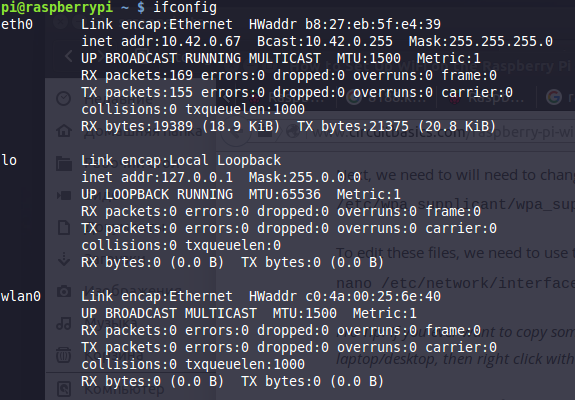
\includegraphics[width=0.6\linewidth]{driver_5}}
\caption{ Результат выполнения команды ifconfig }
\label{driver_5:driver_5}
\end{figure}

\clearpage



